\documentclass{article}
\usepackage[utf8]{inputenc}
\usepackage[margin=1.0in]{geometry}
\usepackage{graphicx}
\usepackage{wrapfig}
\usepackage{amsmath}
\usepackage{caption}
\usepackage[makeroom]{cancel}
\let\vec\mathbf

\title{Convolutional Neural Nets 1}
\author{Alexey Didenkov}
\date{February 6, 2019}

\begin{document}

\maketitle

\section{Introduction}
Convolutional Neural Networks (CNNs) are a type of deep neural networks that have recently seen \textit{large success and widespread usage}. They extend and build onto the plain artificial neural network, but are optimized to \textit{work well with image data}, which makes them conveniently compatible with Computer Vision. This lecture will focus on the \textbf{origin} and \textbf{architecture} of CNNs, with further insight into implementation and applications following in part 2.


\section{Background}
\begin{wrapfigure}{r}{0.35\textwidth}
  \vspace{-50pt}
  \begin{center}
    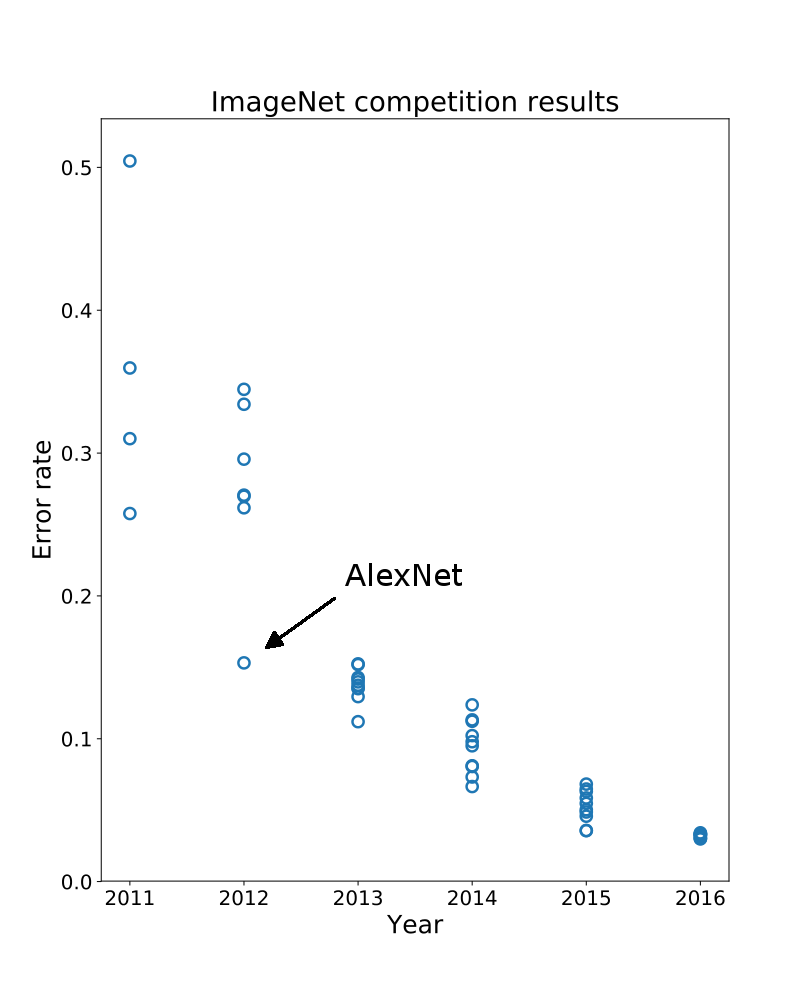
\includegraphics[width=0.35\textwidth]{ImageNet_history.png}
  \end{center}
  \vspace{-25pt}
  \caption{ImageNet Error vs Time}
\end{wrapfigure}
2012. The annual \textbf{ImageNet Large Scale Visual Recognition Challenge} (ILSVRC) was a boxing ring for the toughest CV models that dared to challenge the cutting edge. Everything from wombats and croquet balls to 90 different breeds of dogs—these models promised to classify it all at an error rate of about 25\%—not bad for a dataset of 1000 classes.

Yet, their gradual improvements did not grant them the spotlight that year, for a new challenger has approached. Alex Krizhevsky and his \textbf{CNN} called \textbf{AlexNet} have single-handedly cut the top-5 error to 15.3\%, more than 10.8 percentage points below the previous best (41\% improvement).

The shocking breakthrough brought an abundance of attention and progress to CNNs and Deep Learning, lowering ImageNet error rates to superhuman levels in 2015. More so, it caused an industry-wide Artificial Intelligence boom and kick-started the modern Deep Learning Revolution. As of today, the AlexNet paper has been cited over 35,000 times.


\section{Issues}
Despite the model's phenomenal success, its main contribution was exposure—Krizhevsky has been mainly putting together already existing improvements. These were driven by the goal of resolving various shortcomings of vanilla neural networks, especially those that arise when dealing with images.

\subsection{Excessive Connections}
Imagine that your data consists of square images with a side length of 100px. If you were to process these with a regular neural net, your input layer would consist of $100 \times100=10,000$ neurons. That's $10,000$ connections \textit{for each neuron} in your first hidden layer! If you wanted your hidden layer to be the same size, you'd need a whopping \textit{10 million connections}! This excessive number of connection poses various problems and significantly \textbf{slows down training}. On top of all that, $100 \times100$ is a rather low-quality image by today's standards.

\subsection{Spatial Invariance}
Imagine that you trained a neural network to recognize handwritten digits. The model works perfect as long as you give it the same kind of data that it saw during training—digits that are cropped and perfectly centered. Problem is, digits that are offset or scaled will look completely different to your network—it will be thoroughly confused. You can try to account for that by manually including these modified images in the dataset, but covering for every possible location will blow up the dataset exponentially. Ideally, you want a way to learn what the number '2' looks like, while \textbf{only having to do so once}.

\subsection{Training Time}
Large networks generally get better performance, but they are much more difficult to train. While having to perform this training on a CPU can be annoying today, it was impossible back when CNNs were first developed. A ten-fold increase in performance would be enough to cross the boundary between unfeasible and feasible.


\section{Layers}

\subsection{Convolutional}
As hinted by the name, Convolutional Neural Networks primarily use \textbf{convolutions}. We've already covered these during the Edge Detection lecture—a CNN convolution is basically the same as applying a Gaussian kernel to blur the image or a Sobel kernel to find its edges.
\begin{figure}[!htb]
\centering
\begin{minipage}{0.6\textwidth}
  \centering
  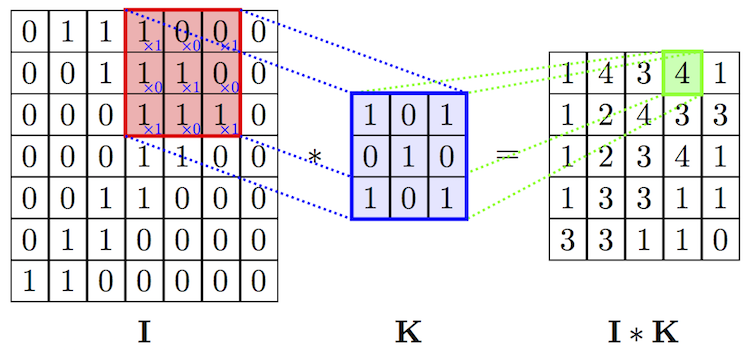
\includegraphics[width=0.9\textwidth]{convolve.png}
  \captionof{figure}{Example of a 2D Convolution}
  \label{fig:test1}
\end{minipage}%
\begin{minipage}{0.4\textwidth}
  \centering
  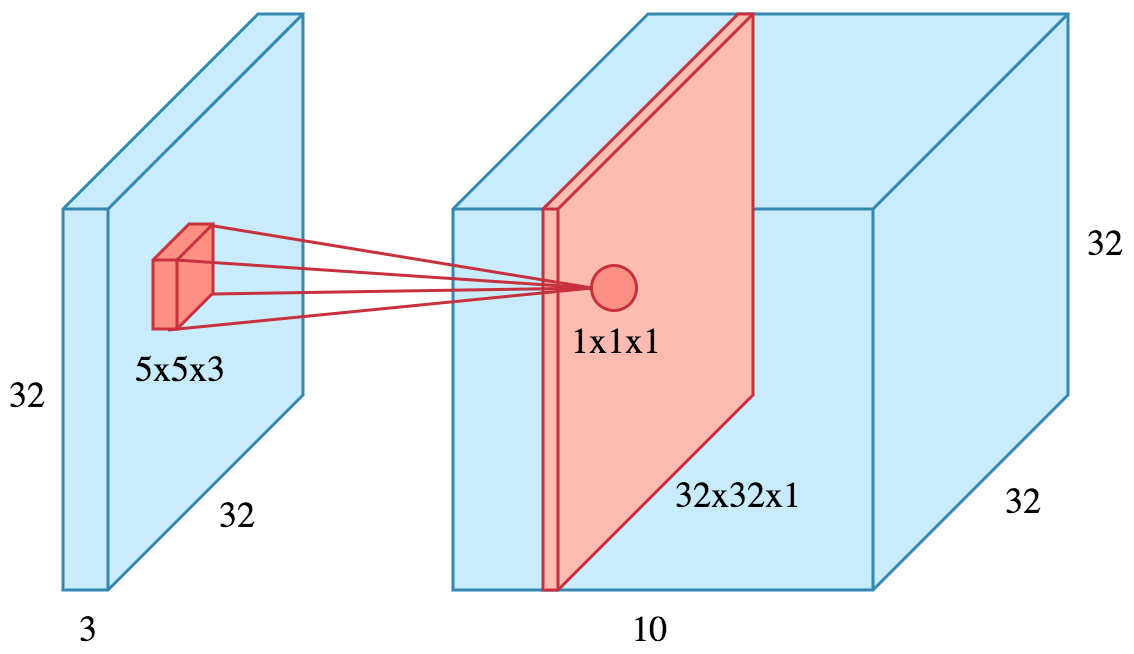
\includegraphics[width=0.9\textwidth]{conv_layer.png}
  \captionof{figure}{Convolutional Layer}
  \label{fig:test2}
\end{minipage}
\end{figure}

Though convolutions were around for a long time, the real breakthrough came when people started \textbf{training kernel values} via gradient descent as opposed to picking them out by hand. Automatically learned weights happen to be the main difference between filters as we know them from CV, and convolutional layers in CNNs.

The very first application of gradient descent to convolutions was in time delay neural networks (TDNNs), where convolutions were applied over the time dimension. The first modern-like CNN was developed by Yann LeCun, who used backpropagation to learn better kernels in a convolutional system aimed at recognizing hand-written ZIP-codes. This model, called \textbf{LeNet}, was developed in 1989.

\subsubsection{Motivation and Intuition}
Similar to how plain neural networks drew inspiration from biological neurons, so did CNNs. The latter primarily focused on 1950s and 1960s studies by Hubel and Wiesel on monkey and cat brains. The main insights are as follows:
\begin{enumerate}
    \item Neurons have a very specific \textbf{receptive field} they are in charge of. Neurons typically analyze information that is spatially close, instead of combining signals from different ends of an animal's field of vision.
    \item There are two different types of cells: \textbf{simple}, which respond to straight edges of varying orientations, and \textbf{complex}, which are insensitive to the exact position of edges over larger receptive fields.
\end{enumerate}
It's clear how 2D convolutions play into these characteristics. Neurons in the first hidden layer have a receptive field equivalent to the kernel size—these neurons are completely blind to any pixel values that don't fall under the filter. Neurons in the second hidden layer will be affected if any of the first-layer neurons change, which together are affected by changes over a larger area. Thus, successive layers don't only extract more complex information, but also \textit{respond to a larger receptive field}, making them similar to complex neurons in actual brains.
\subsubsection{Local Connectivity and Arrangement}
While convolutions can appear very different from regular neural network layers, thinking of them as such reveals how they solve the \textbf{excessive connections issue}. In a regular layer, every node in the second layer is connected via a unique weight to \textit{every neuron} in the first. The main differences of convolutional layers are:
\begin{enumerate}
    \item \textbf{Local connections}—From biology, we gain the insight that neurons should only consider a small neighborhood around them. We can thus assume that data typically have local significance, i.e. there is no point in giving every neuron access to pixel values from opposite corners of the original image. Instead of receiving all $10,000$ input values, each neuron after a $5\times5$ convolution only needs the $25$ values most relevant to it. If our assumption is correct, neurons in regular networks should by default learn to ignore everything but a small neighborhood. We are just making their (and our) job easier by removing these connections in the first place, leveraging our knowledge of the pixels' \textbf{spatial relation} to each other.
    \item \textbf{Shared weights}—These $25$ values coming to each neuron are multiplied by some weights, arranged in a $5\times5$ kernel. However, this kernel is exactly the same for each neuron in the next layer, the only thing changing is the region over which it is applied. First of all, this additionally reduces the total number of parameters. Most significantly, though, it gives the network \textbf{spatial invariance}. To learn to recognize edges, a CNN only has to learn the Sobel kernel once, at which point it will be applied to all raw pixel values. Similarly, if a more complex filter learns to detect the digit '2', it will not be able to do so independent of where this '2' appears in the image.
\end{enumerate}
\subsubsection{GPU Acceleration}
Much of the reason why CNNs stayed obscure during their discovery in the 1980s were the limitations to computational power that made them impractical. Still, their widespread use owes thanks to another major development—the use of \textbf{GPUs}. In the late 2000s and early 2010s various researchers have demonstrated that convolutions can be significantly sped up when forward- and back-propagation through convolutions is done in parallel. Achieving speedup factors of \textbf{20 to 60}, these researchers have entered their CNNs into various competitions, for the first time achieving superhuman performance.

\subsection{Subsampling}
Convolutional layers have the ability to apply multiple filters to an image through a single operation. However, the "image size" of the data stays the same. To broaden receptive fields and encourage spatial invariance, we need to ideally reduce the image size.

This can be done by making convolutions have a larger \textbf{stride size}, which is equivalent to skipping some of the neurons on each layer. Although it seems like we're throwing information away, it is more or less perserved as long as kernel sizes are larger than step sizes.

In practice, however, we typically want to perform many convolution operations before reducing the image size (the latter is difficult to undo). So, convolutional layers are typically \textbf{padded} to ensure that they keep image size identical, while special \textbf{subsampling levels} are created for the sole purpose of reducing the image size. Currently, the most common type is \textbf{max-pooling}, where a sliding window (typically $2\times2$ with a step size of $2$) extracts the maximum value at each location.
\begin{figure}[!htb]
\centering
\begin{minipage}{0.6\textwidth}
  \centering
  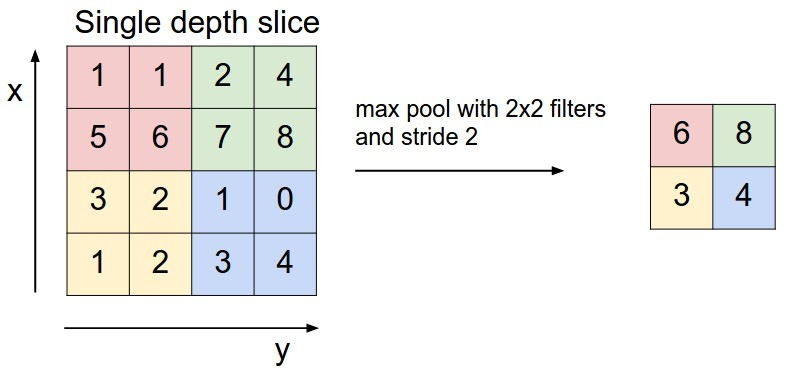
\includegraphics[width=0.9\textwidth]{maxpool.jpeg}
  \captionof{figure}{Example of max-pooling}
  \label{fig:test3}
\end{minipage}%
\begin{minipage}{0.4\textwidth}
  \centering
  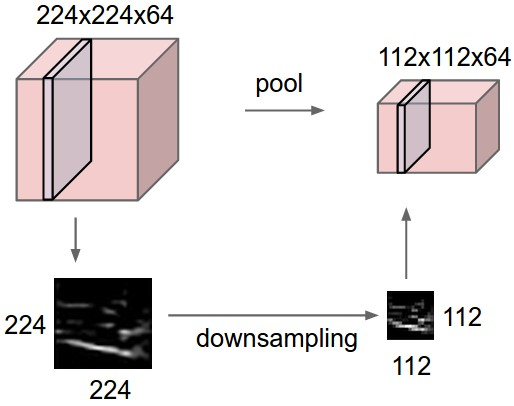
\includegraphics[width=0.9\textwidth]{pool_layer.jpeg}
  \captionof{figure}{Pooling Layer}
  \label{fig:test4}
\end{minipage}
\end{figure}

\subsubsection{Controversy}
Plenty of people dislike the commonly used max-pooling layer and think we can get rid of it. They have valid reasons—though the layer makes the network translationally invariant it also \textit{loses spatial information}, which additionally complicates backpropagation and unpooling.

As previously mentioned, pooling layers are similar to performing convolutions with a larger stride length. A 2015 study found that an \textbf{All Convolutional Net} created by such replacements achieves comparable performance.

The same goal of removing the pooling layer motivated Geoffrey Hinton, one of the pioneers of deep learning (coincidentally, Alex Krizhevsky's PhD advisor), to create \textbf{Capsule Networks}. Despite their numerous advantages, however, these networks fall short of the state-of-the-art. Even if theoretically flawed, pooling layers remain hard to beat in practice.

\subsection{Fully Connected}
To complete the task of classification, most CNNs typically use \textbf{dense layers}, or \textbf{fully connected layers}. These terms both refer to the connection layers found in typical neural networks, mainly to distinguish them from other layers (convolutional, subsampling).

\subsection{Putting it All Together}
Despite CNNs existing in the ready state for over two decades before their popularization, it took numerous iterations of Moore's Law and various efforts of GPU optimization to get them to a practical state. Even then, attention only came when everything was put together and displayed under the spotlight, in what was basically the CV Olympics.

Likewise, here is the full CNN architecture:

\begin{figure}[!htb]
  \centering
  \vspace{-3pt}
  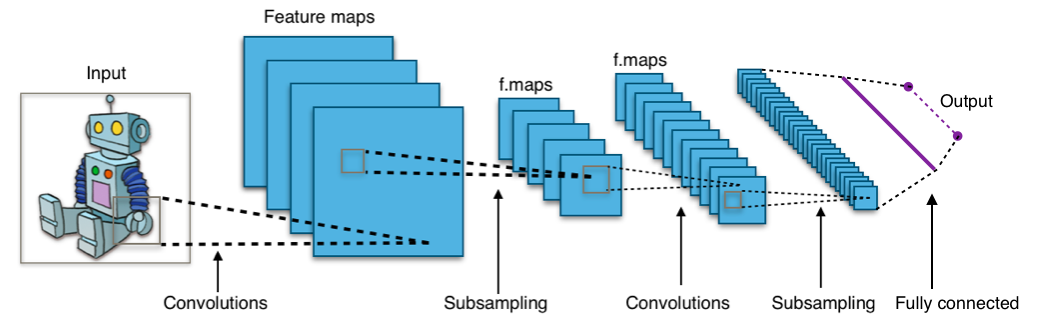
\includegraphics[width=1.0\textwidth]{cnn.png}
  \vspace{-5pt}
  \captionof{figure}{Example of a Full CNN Architecture}
  \vspace{-20pt}
\end{figure}

% \section{State of the Art}
% \begin{wrapfigure}{r}{0.35\textwidth}
%   \vspace{-50pt}
%   \begin{center}
%     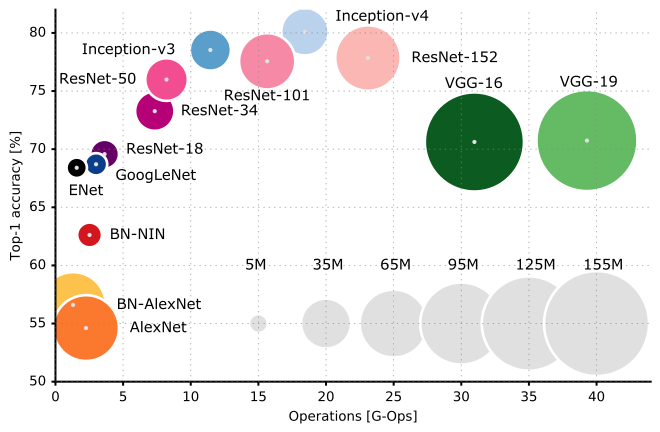
\includegraphics[width=0.35\textwidth]{state-of-the-art.png}
%   \end{center}
%   \vspace{-25pt}
%   \caption{ImageNet Error vs Time}
% \end{wrapfigure}
% Examples + visual
% Conclusion

\end{document}
